\section{Implementing Device Algorithms} 
\label{sec:device models}
Due to the limited sensing capability of ICDs, device manufacturers have developed different algorithms to identify the electrical events and correctly diagnose the cardiac arrhythmia as being \ac{VT} or \ac{SVT}.
In this paper we implemented the detection algorithm Rhythm ID of Boston Scientific \cite{compass,Ellenbogen11_Pacingbook},% [???Compass, pacingdefibrillation,VTC paper, ICD book, Ellenbogen].
and PRLogic+Wavelet (PRL+W) of Medtronic \cite{Singer,Wavelet}.
%In available literature on the evaluations of device algorithms descriptions of the device algorithms are not detailed enough for full implementation.
%To obtain the detailed implementation we further reviewed clinical execution traces from literature like \cite{Singer} to infer detailed executions of the algorithms. 
We also set up a testing platform to validate our implementations against real ICDs using conformance testing.

\section{ICD Sensing}
\label{sec:sensing}
\begin{figure}[t]
	\centering
	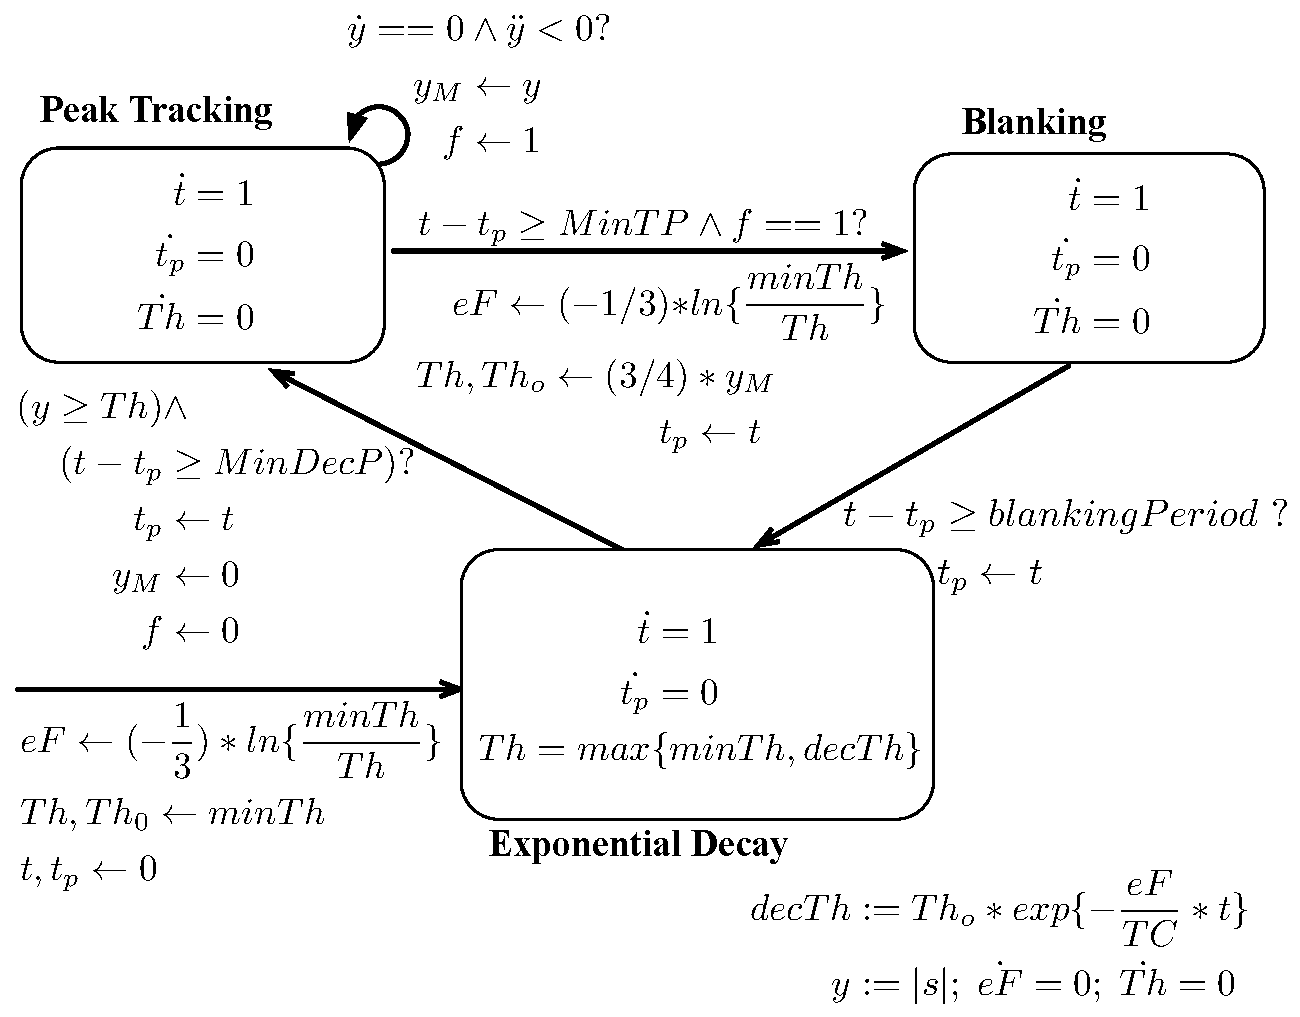
\includegraphics[scale=0.35]{figures/sensingModel}
	\vspace{-10pt}
	\caption{\small $\Sys_{Sense}$. States not shown in a mode have a 0 derivative, e.g., $\dot{eF}=0$ in all modes.}
	\vspace{-10pt}
	\label{fig:sensingModel}
\end{figure}
\begin{figure}[t]
	\centering
	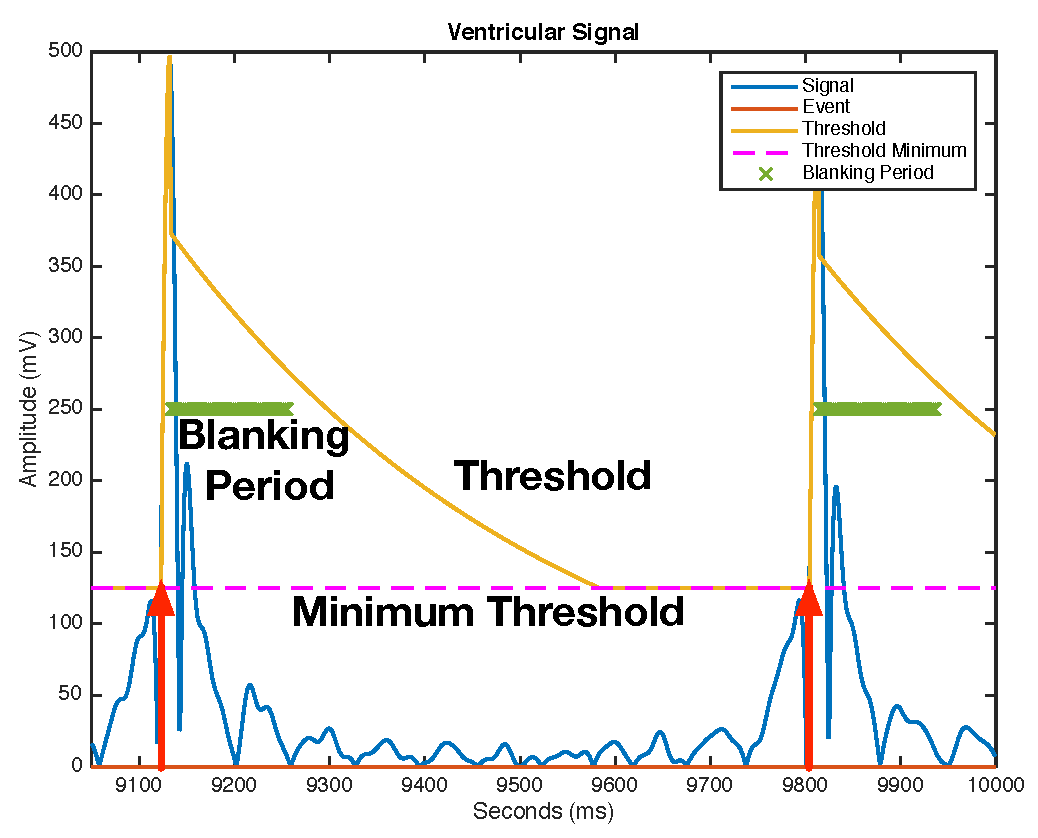
\includegraphics[scale=0.3]{figures/sensingExample}
	\vspace{-10pt}
	\caption{\small Example of dynamic threshold adjustment in ICD sensing algorithm. The shown signal is rectified.}
	\vspace{-10pt}
	\label{fig:sensingExample}
\end{figure}

\emph{Sensing} is the process by which cardiac signals $\egm$ measured through the leads of the \ac{ICD} are converted to cardiac timing events.
The \ac{ICD} sensing algorithm is a threshold-based algorithm which declares events when the signal exceeds a dynamically-adjusted threshold $Th$.
%The threshold is dynamically adjusted in order to operate robustly in complex environments where cardiac events can vary greatly in signal amplitude and frequency, such as during \ac{VF}.

Fig. \ref{fig:sensingModel} shows the model $\Sys_{Sense}$ of the sensing algorithm, and Fig. \ref{fig:sensingExample} illustrates its operation. 
%In Fig. \ref{fig:overview} (ICD Sensing - $\Sys_{Sense}$), states not shown in a mode have a 0 derivative, e.g., $\dot{eF}=0$ in all modes. $y(t) = |\egm(t)|$.
The sensing takes place on the rectified \ac{EGM} signal $y = |\egm|$.
After an event is declared at the current threshold value ($y(t)\geq Th(t)$ in Fig. \ref{fig:sensingModel}), the algorithm tracks the signal in order to measure the next peak's amplitude \yhl{(Peak Tracking)}.
%During transition, the state to indicate peak discovery is reset ($f=0$). 
For a duration $MinTP$ (min tracking period) the latest peak is saved in $y_M$.
A variable $f$ indicates that a peak was found.
After a peak is found ($f==1$) and after the end of the tracking period, the algorithm enters a fixed \emph{Blanking Period} \yhl{(Blanking)}, during which additional events are ignored.
\yhl{On the transition to Blanking}, $Th$ and $Th_0$ are set to 3/4 the current value of $y_{M}$ and the exponential factor of decay is updated ($eF=(-1/3)*ln{\frac{minTh}{TH}}$). 
At the end of the blanking period, the algorithm then transitions to the Exponential Decay mode in which $Th$ decays exponentially from $Th_0$ to a minimum level \yhl{(Exponential Decay)}:
$Th(t) = \max(minTh, Th_0\cdot exp(-(eF/TC)t)) $.
The algorithm stays in the Exponential Decay mode for at least a sampling period of $MinDecP$.
Correspondingly, there is a de facto Maximum Decay Period $MaxDecP$ after which the system transitions again to PeakTracking since the signal $y$ is bound to exceed the minimum threshold $minTh$.
Different manufacturers may use a step-wise decay instead of exponential, but the principle is the same.
%
Local peak detection is modeled via the $\dot{y} = 0 \wedge \ddot{y}<0$ transition.
While $y=|\egm|$ is non-differentiable at 0, the peak will occur away from 0, as shown in Fig. \ref{fig:sensingExample}.
The other states in Fig. \ref{fig:sensingModel} are $t, t_p$ (clocks).
$minTh$ and $TC$ are constant parameters.
\begin{thm}
	\label{thm:sensing}
	$\Sys_{Sense}$ is STORMED.	
\end{thm}
\begin{prf}
	\textbf{(S)} By definition, we only need to consider transitions between different modes to establish separability. 
	For all such transitions, there is a minimum dwell time in the mode before taking the transition, namely $MinTP$ in PeakTracking, $BlankingPeriod$ in Blanking, and  $MinDecP$ in mode ExponentialDecay.
	So the system is separable since there is a uniform minimum flow before jumping.
	\\
	\textbf{(T)} Flows are either constant, (piece-wise) linear, or piece-wise linear and exponential (in the case of $y$ and its derivatives) and therefore are TISG.
	\\
	\textbf{(O)} All the flows, resets and guard sets are definable in $\Lc_{\exp}$.
	(The absolute value and $\max$ functions can be broken down into boolean disjunctions of definable functions, and $t \mapsto \ln(t)$ is o-minimal by o-minimality of $\exp$).
	\\
	\textbf{(RM)} The state is $x = (t, t_p, y, y_M, f, Th, Th_0,eF) \in \Re^8$, and let 
	 $\phi = (\phi_t, \phi_{p}, \phi_y, \phi_m, \phi_f, \phi_{Th},\phi_0,\phi_{eF})$ be the corresponding $\phi$ vector.
	Recall that the \ac{EGM} voltage $\egm$, and so $y=|s|$, is upper-bounded by $V_M$.	
	\\ 
	\textbf{ExponentialDecay $\rightarrow$ PeakTracking}.
	Only $t_p,y_M$ and $f$ are modified, so monotonicity produces the constraint
	 $\phi_p(t-t_p) +\phi_m(0-y_M) + \phi_f(0-1) \stackrel{Want}{\geq} \varepsilon (|t-t_p|+|y_M|+1)$.
	We require the stronger constraint to hold:
	\[\phi_t MinDecP - \phi_m V_M -\phi_f \stackrel{Want}{\geq} \varepsilon(MaxDecP + V_M+1)\]
	\\
	\textbf{PeakTracking $\rightarrow$ PeakTracking}. Only $y_M$ and $f$ are reset. 
	Algebraic manipulation yields $-2V_M\phi_m + \phi_f \stackrel{Want}{\geq} \zeta$
	\\
	\textbf{PeakTracking $\rightarrow$ Blanking}.
	$t_p,eF,Th$ and $Th_0$ are reset, so we get
	\begin{eqnarray*}
	&&\;\phi_p(t-t_p) + \phi_{eF}(-(1/3)\ln(minTh/Th)-eF) 
	\\
	&&+\phi_{Th}(3y_M/4-Th) +\phi_0(3y_M/4-Th_0)
	\\
	&&\geq \varepsilon(|t-t_p|+ |-\frac{1}{3}\ln(\frac{minTh}{Th})-eF|
	\\
	&&+|\frac{3y_M}{4}-Th|+|\frac{3y_M}{4}-Th_0|)
	\end{eqnarray*}
	
	$Th$ is lower-bounded by $minTh$ at all times, and it is naturally upper-bounded by $V_M$ as the threshold should never exceed the largest possible attainable voltage. 
	By the same token, $0\leq eF \leq (1/3)\ln(V_M/minTh)$.
	Then we want the stronger inequality
	\begin{eqnarray*}
	\phi_p MinTP &+& \phi_{eF}(0-(1/3)\ln(V_M/minTh)
	\\
	&+&\phi_{Th}(-V_M) +\phi_0(-V_M)
	\\
	&\geq& \varepsilon(MaxTP+ |\frac{1}{3}\ln(\frac{V_M}{Th})|+|V_M|+|V_M|)
	\end{eqnarray*}
	\\
	\textbf{Blanking $\rightarrow$ ExponentialDecay}. Only $t_p$ is reset and therefore we want, $\phi_p(t-t_p) \geq \varepsilon(|t-t_p|)$, thus the transition yields $\phi_p \geq \varepsilon$.
	
	The above equations can be simultaneously satisfied.
	The simplest thing would be to set all $\phi$ terms that appear above to 0 except for $\phi_t,\phi_p$ which are calculated accordingly.
	
	The flows can be shown to be monotonic along the same $\phi$ and with the same $\varepsilon$.
	For example, in mode ExponentialDecay, only $t,y$ and $Th$ flow.
	Making use of the $V_M$ bound on $y$, we get the constraint
	$\phi_t \tau - 2V_M\phi_y +\phi_{Th}(Th(t+\tau)-Th(t))\geq \varepsilon(\tau+2V_M + |Th(t+\tau)-Th(t)| )$, 
	which yields $\phi_t \geq \varepsilon$, $\phi_y \leq -\varepsilon$ and $\phi_{Th} \geq \varepsilon$. 
	Similarly for the rest.	
\end{prf}

%\begin{thm}
%\label{thm:sensing}
%$\Sys_{Sense}$ is STORMED.	
%\end{thm}
%\begin{prf}
%\textbf{(S)} The guards are separable since each mode has only one guard.
%\\
%\textbf{(T)} The flows are constant, linear or equal to $\pm \egm(t)$ (in the case of $y$) and so are TISG.
%\\
%\textbf{(O)} All the flows, resets and guard sets are definable in $\Lc_{\exp}$.
%(The absolute value and $\max$ functions can be broken down into boolean disjunctions of definable functions).
%In particular, $t \mapsto \ln(t)$ is o-minimal by o-minimality of $\exp$.
%\\
%\textbf{(RM)} The only reset happens on the PeakTracking $\rightarrow$ Blanking transition. 
%The state is $x = (t,Th, eF,Th_0,t_p,y) \in \Re^5$.
%We seek a vector $\phi = (\phi_t, \phi_{Th}, \phi_{eF},\phi_0,\phi_y)$ and $\varepsilon >0$ s.t. 
%\begin{equation}
%\label{eq:sense rm}
%\phi \cdot \left(\begin{matrix}
%t-t \\ (3/4)Th-Th\\ -(1/3)\ln(minTh/Th) - eF\\ (3/4)Th-Th_0\\ t-t_p \\ y-y
%\end{matrix}
%\right) \defeq \phi \cdot \delta \stackrel{Want}{\geq} \varepsilon ||\delta||
%\end{equation} 
%$Th$ is lower-bounded by $minTh$ at all times, and it naturally has an upper bound, since it doesn't make sense to set it above the largest possible voltage. 
%Let that maximum be $maxTh$.
%Then we want the stronger inequality
%\begin{eqnarray*}
%&&\phi_{Th}(-Th/4) + \phi_{eF}(-(1/3)ln(minTh/Th)-eF) 
%\\
%&+& \phi_0(3Th/4-Th_0) + \phi_t (t-t_p) \geq ||\delta||
%\\
%&\geq& -\frac{\phi_{Th}}{4}maxTh + \phi_{eF}(-\frac{2}{3}\ln(minTh/Th)) 
%\\
%&& -\phi_0(2maxTh) + \phi_p(t-t_p)
%\\
%&\stackrel{Want}{\geq}& \varepsilon \left(|\frac{maxTh}{4}| + |\frac{2}{3}\ln(\frac{minTh}{Th})| + |2maxTh| +  \phi_p|t-t_p|\right)
%\end{eqnarray*}
%Since the $\ln$ term is negative and $t\geq t_p$,this yields the constraints:
%$\phi_0,\phi_{Th} < -\varepsilon \text{  and  } \phi_{eF},\phi_t > \varepsilon$.
%%\begin{equation}
%%\label{eq:constraint sense rm}
%%\phi_0,\phi_{Th} < -\varepsilon \text{  and  } \phi_{eF},\phi_t > \varepsilon
%%\end{equation}
%
%The flows are also monotonic along the same $\phi$ and with the same $\varepsilon$.
%For any $t,\tau>0$ and $x\in \stSet$, flow monotonicity is implied by the stronger inequality
%\begin{equation}
%\label{eq:sense fm}
%\phi \cdot \left(\begin{matrix}
%t+\tau-t \\ Th-Th\\ eF - eF\\ Th_0-Th_0\\ t_p-t_p \\ |\egm(t+\tau)|-|\egm(t)|
%\end{matrix}
%\right) \stackrel{Want}{\geq} \varepsilon (\tau + \underbrace{||\egm(t+\tau)|-|\egm(t)||}_{\delta \egm})
%\end{equation} 
%$\implies \phi_t \tau + \phi_y (|\egm(t+\tau)|-|\egm(t)|) \geq \varepsilon (\tau + \left| |\egm(t+\tau)|-|\egm(t)| \right| )$
%Therefore we can choose $\phi_t > \varepsilon$ as before and $\phi_y < -\varepsilon$.
%%We show this for Mode 1 only, the other modes are dealt with similarly.
%%\underline{Mode 1.} For any $t,\tau>0$ and $x\in \stSet$, flow monotonicity 
%%$\phi\cdot(\theta(t+\tau;x)-\theta(t;x)) \geq \varepsilon ||\theta(t+\tau;x)-\theta(t;x)||$ is implied by the stronger inequality
%%\begin{equation}
%%\label{eq:sense fm}
%%\phi \cdot \left(\begin{matrix}
%%t+\tau-t \\ Th-Th\\ eF - eF\\ Th_0-Th_0\\ t_p-t_p \\ -\egm(t+\tau)+\egm(t)
%%\end{matrix}
%%\right) \stackrel{Want}{\geq} \varepsilon (\tau + \underbrace{|\egm(t)-\egm(t+\tau)|}_{\delta \egm})
%%\end{equation} 
%%Observing that the \ac{EGM} signal $\egm$ has naturally defined minimum $\egm_{min}$ and maximum $\egm_{max}$, \eqref{eq:sense fm} is further implied by 
%%\begin{equation}
%%\phi_t\tau + \phi_y(\delta \egm) \geq \phi_t \tau - \phi_y(s_{min} -  s_{max}) \stackrel{Want}{\geq} \varepsilon (\tau +|s_{min} -  s_{max}|)
%%\end{equation}
%%which yields the constraints $\phi_t > \varepsilon, \phi_y < -\varepsilon$, which are consistent with \eqref{eq:constraint sense rm}.
%%The flow monotonicity constraints from the other modes are similarly consistent with \eqref{eq:constraint sense rm}. 
%\end{prf}

\subsection{VT Detection Algorithm}
\label{sec:svtvt}
%The limited sensing resolution and noise in the \ac{EGM} signals make it is impossible for the device to achieve 100\% accuracy for SVT/VT discrimination.
Device companies have developed different algorithmic components to distinguish \ac{SVT} from \ac{VT}, referred to as \emph{discriminators}. 
Each discriminator utilizes the history of timing and/or morphology of the EGM signals to determine whether the current rhythm is a \ac{VT} or \ac{SVT} (or neither).
%The decisions of each discriminators are then combined using a decision tree structure to decide whether to deliver or inhibit therapy.
No single discriminator is sufficient on its own to discriminate between \ac{SVT} and \ac{VT}, because these classes of arrhythmias can appear similar in a number of criteria.
Therefore discriminators are organized in a decision tree.%, as illustrated in Fig. \ref{fig:BS_det}.
We have implemented the detection algorithms Rhythm ID from Boston Scientific and PRL+W from Medtronic. 
This section gives an overview of both algorithms.

%We will need the following definition: an \emph{interval} is the amount of time between two consecutive electrical events. 
%Thus a ventricular interval is the duration between two ventricular events.
%Intervals are variable in length. 
%Consistently short intervals imply a fast rhythm.

\begin{figure*}[t]
	\centering
	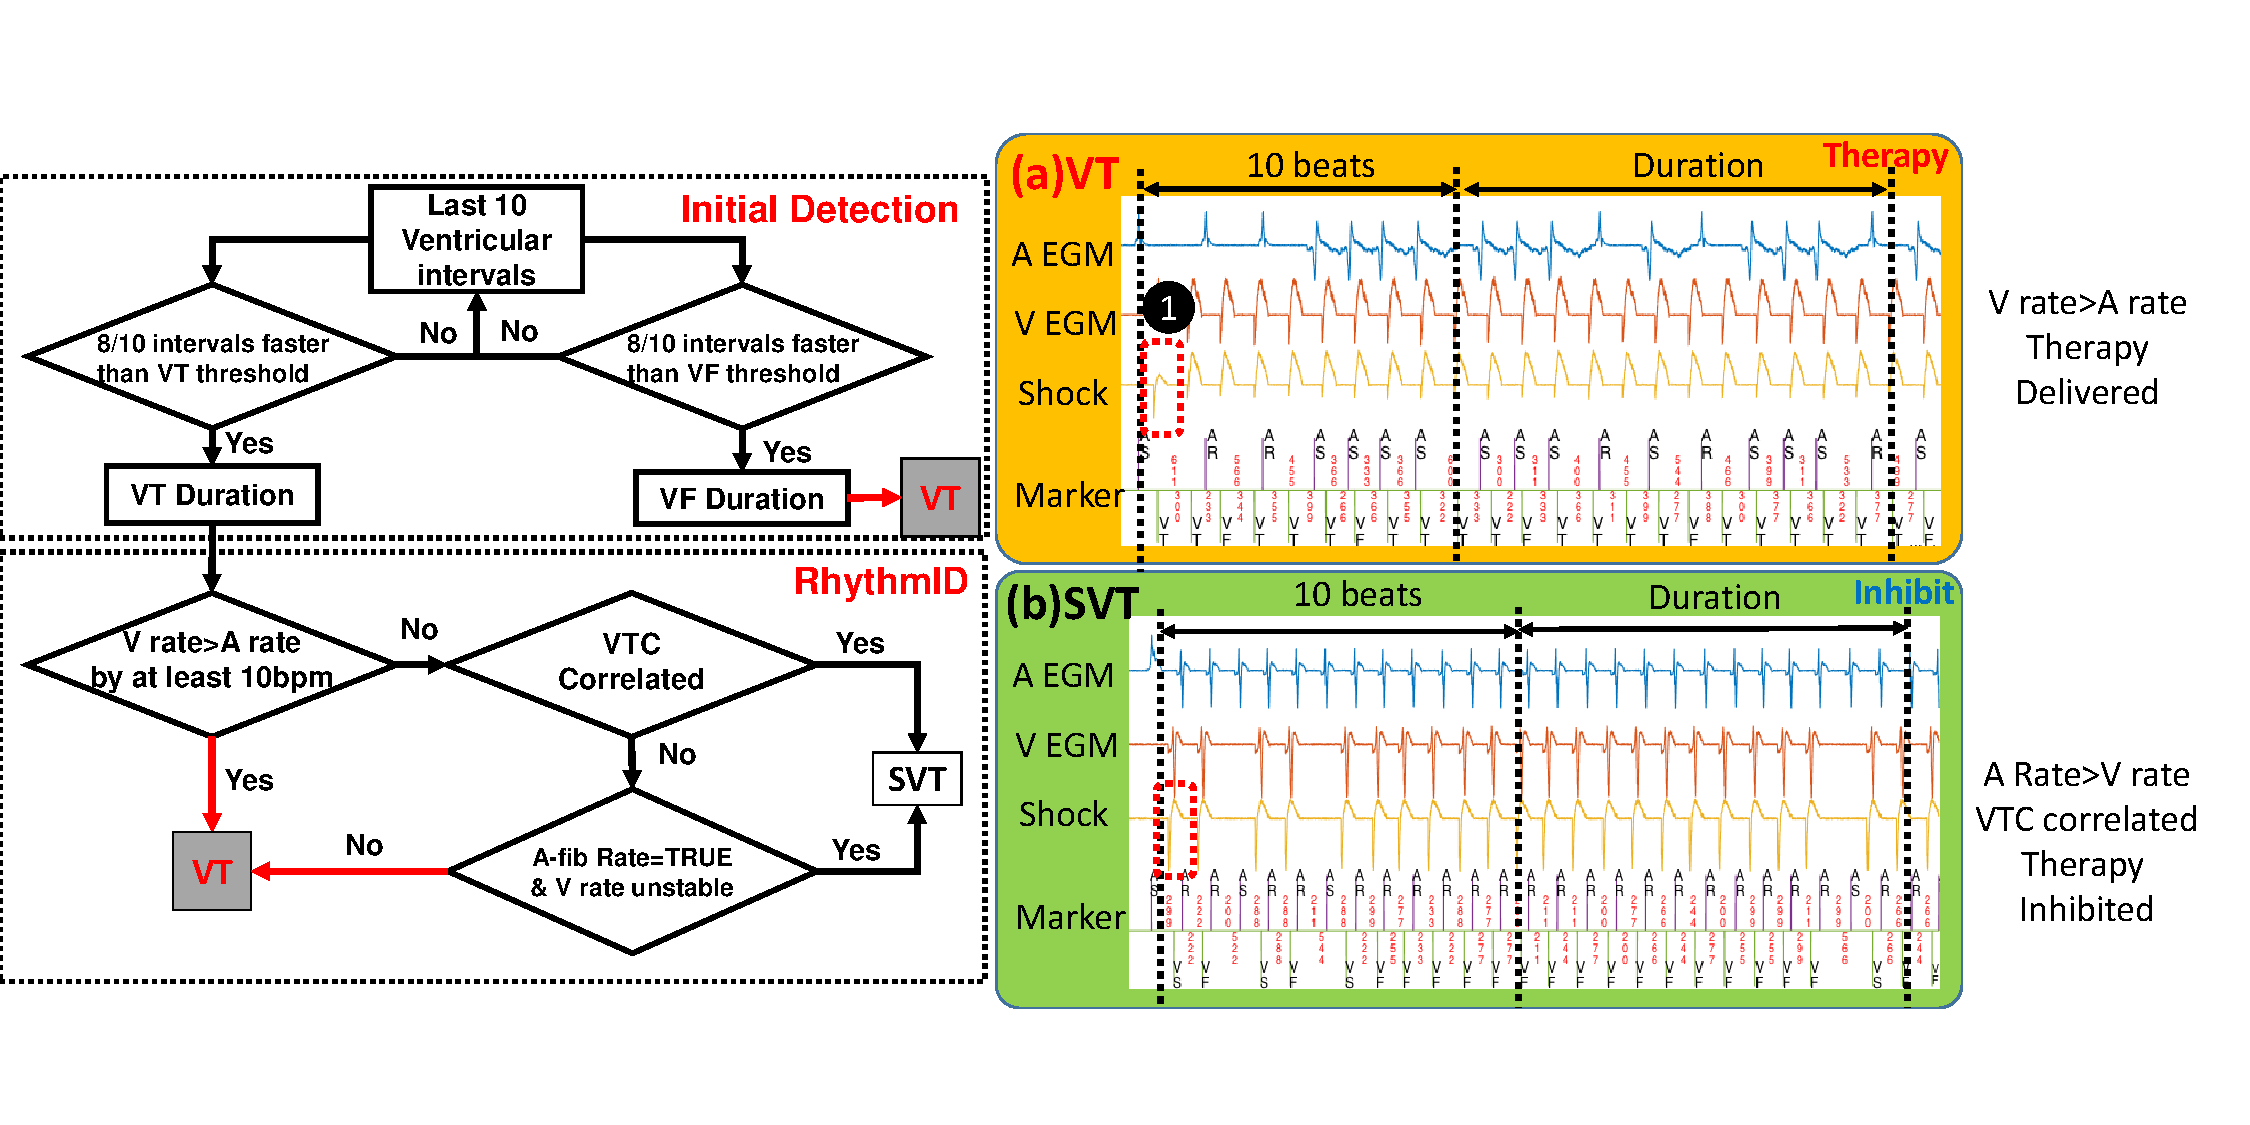
\includegraphics[scale=0.38]{figs/BS_det.pdf}
	\vspace{-10pt}
	\caption{\small SVT/VT detection algorithm by Boston Scientific \cite{compass}. The two cases on the right illustrate two different decisions by the algorithm. (a) illustrates a sustained VT case where at the end of the Duration, the ventricular rate is faster than the atrial rate. The algorithm correctly identified the rhythm as VT and delivered therapy. (b) illustrates a SVT case where at the end of the Duration, the ventricular rate is slower than the atrial rate. Then by comparing the EGM morphology in the Shock channel (Marker 1) with the stored NSR template (Marker 2) for the last 10 EGM events, the algorithm decided that the morphology is correlated, therefore therapy is inhibited.}
	\label{fig:BS_det}
\end{figure*}

\subsubsection{Rhythm ID}
Rhythm ID's decision tree is shown in Fig.~\ref{fig:BS_det}.
Rhythm ID detects an episode by continuously examining the last 10 ventricular intervals and comparing them with VT and VF thresholds. 
If 8/10 intervals are shorter than the VF threshold for a certain pre-set \emph{VF Duration} (e.g., 2.5 seconds) then the algorithm declares VF.
Otherwise, if 8/10 intervals are shorter than the VT threshold for a certain VT Duration, then further discriminators are used.
First, if the ventricular rate is greater than the atrial rate for the last 10 ventricular beats, Rhythm ID will determine the condition is VT.
Otherwise, the Vector Timing and Correlation (VTC) discriminator~\cite{VTC} compares EGM morphology of the last 10 ventricular events with an EGM \emph{template} saved during \ac{NSR}.
VTC is based on the assumption that the EGM morphology of the shock channel during VT is different from its morphology during SVT and NSR.
If the correlation between the current EGM's morphology and the stored NSR morphology is above a pre-set threshold, the current rhythm is more likely to be SVT than VT, and therapy is withheld.
Otherwise, if the atrial rate is equal to a pre-set fibrillation rate and the variance of the ventricular interval length exceeds a certain limit, the algorithm decides it's an \ac{SVT}. 
Otherwise, it decides this is a \ac{VT}.
%As shown in Fig. \ref{fig:BS_det}(b), at the end of the duration, the atrial rate is faster than the ventricular rate. 
%The morphology in the shock channel is similar to the NSR morphology (red dashed) so VTC is correlated and therapy is inhibited.
%As a comparison the morphology during VT is different from the NSR morphology (Marker 1 in Fig. \ref{fig:BS_det}).

\subsubsection{PR Logic+Wavelet}
PRL+W also utilizes rate-based and morphology-based discriminators similar (but not identical) to Rhythm ID.
The morphology discriminator used in PRL+W  is similar to VTC in Rhythm ID, but operates in the wavelet domain~\cite{Wavelet}.
PRL+W also continuously compares the pattern of atrial and ventricular activation to 19 pre-defined patterns~\cite{Singer}.
Each pattern is associated to a heart condition, like Sinus Tachycardia or \ac{VT}.
A match between the current activity and one of the pre-defined patterns is used as an indication that the current rhythm is explained by the associated condition.


\subsection{Validation}
\label{sec:validation}
%\begin{figure}[t]
%	\centering
%	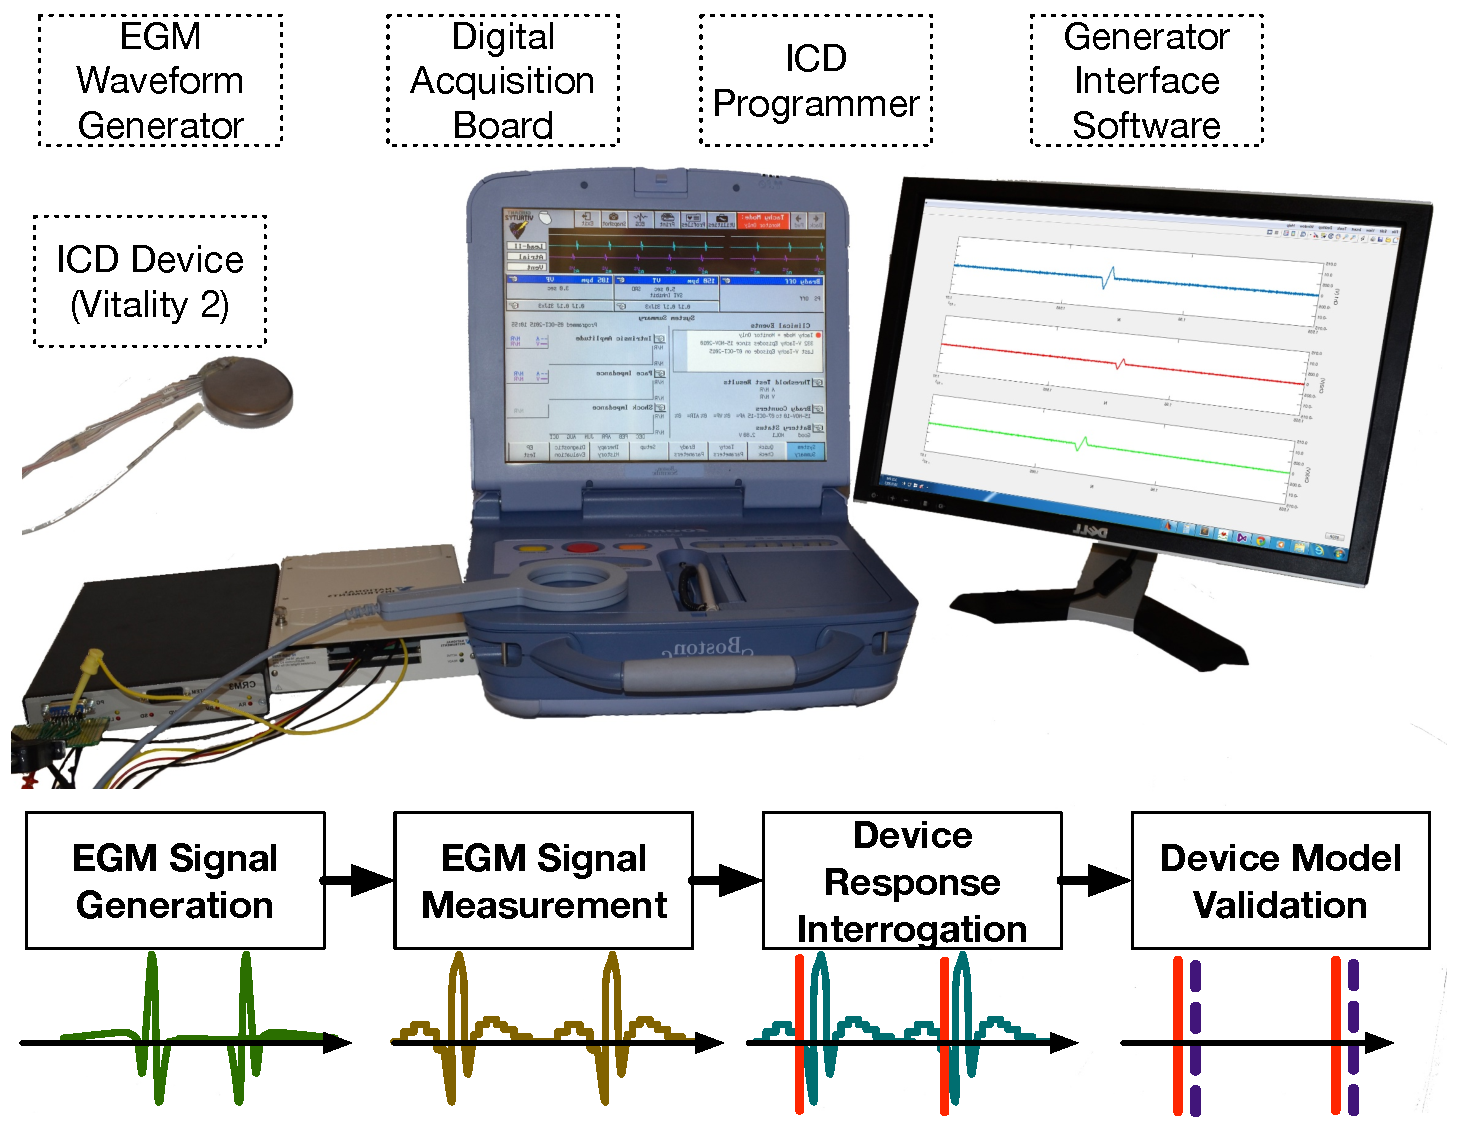
\includegraphics[scale=0.28]{figures/figValidationSetup.pdf}
%	\vspace{-10pt}
%	\caption{\small Model Validation. 14 different scenarios were generated from the EGM waveform generator for Boston Scientific and input into the Vitality 2 ICD. The input signal was acquired through the DAQ board and applied to the device model implementation. The ICD response was interrogated using the ICD programmer and compared to the output of the device model.}
%	\vspace{-10pt}
%	\label{fig:validationSetup}
%\end{figure}
\begin{figure}[t ]
	\centering
	\includegraphics[scale=0.28]{figures/figScreenshot.pdf}
	\caption{\small Example of validation output screenshots (Ventricular fibrillation) showing matching therapy decision for the ICD and our implementation.}
	\vspace{-10pt}
	\label{fig:validation}
\end{figure}

Conformance testing was used to validate the software implementations of the Vitality II device by Boston Scientific. 
The validation hardware setup is illustrated in Fig.~\ref{fig:validation}. 
14 different scenarios were specified and programmed into an EGM Waveform generator (CRM3 Simulator, Guidant, USA) such that it would output a signal to the connected Vitality II device.
The various scenarios traverse 7 out of 9 branches of the detection algorithm for Boston Scientific described in Sec. \ref{sec:svtvt} and shown in Fig. \ref{fig:BS_det}. 
The response of the \ac{ICD} interrogated using an ICD programmer (ZOOM Latitiude, Boston Scientific).
As the waveform was applied to the ICD, the waveform was simultaneously acquired using a National Instruments \ac{DAQ} board.
The recorded waveform was then applied to the device model and response was compared.
Fig. \ref{fig:validation} shows an example of one such scenario, specificallly \ac{VF}. 
In this case, the software model matched to the decision of the actual \ac{ICD} which also determined that therapy should be applied.

In all scenarios, the decision of model conformed to that of the \ac{ICD}. 
The remaining two branches were not reachable due to the limited output capability of the programmer.
The Medtronic software implementation can be validated using a similar process.
